% Lead: James Mullaney
%The Data Products that could be produced were strongly dependent on the type and quality of the data collected during the on-sky commissioning campaign.
%This section should also describe clearly  which columns are not yet available in DP1 from the baseline schema
%Link to the online schema for DP1. Explain what is not there and if known an expected release timescale. Maybe also include a static extract in an appendix.
\section{Overview of the contents of Rubin DP1
\label{sec:data_products}}
%\james{All parts, aside from the Solar System Data Products are ready for review. I also need to get to the bottom of why some of the numbers don't reconcile, so please review the text, rather than the numbers.}

Here we describe Rubin \gls{DP1} data products and provide summary statistics for each.
The \gls{DP1} science data products are derived from the \nvisitimages individual \gls{CCD} images taken across \nexposures exposures in the \nfields \gls{LSSTComCam} commissioning fields (\secref{ssec:pipelines_commissioning}).

The data products that comprise \gls{DP1} provide an early preview of future LSST data releases and are strongly dependent on the type and quality of the data that was collected during \gls{LSSTComCam} on-sky campaign (\secref{ssec:pipelines_commissioning}).
Consequently not all anticipated  \gls{LSST} data products, as described in the \gls{DPDD} \citep{LSE-163} were produced for the \gls{DP1} dataset.

Rubin Observatory has adopted the convention by which single-epoch detections are referred to as Sources.
By contrast, the astrophysical object associated with a given detection is referred to as an Object.
\footnote{We caution that this nomenclature is not universal; for example, some surveys call ``detections'' what we call ``sources'', and use the term ``sources'' for what we call ``objects''.}
As such, a given Object will likely have multiple associated  Sources, since it will be observed in multiple epochs.

At the highest level, the \gls{DP1} data products fall into one of five types:
\begin{itemize}
\item \textbf{Images}, including single-\gls{epoch} images, deep and template coadded images, and difference images;
\item \textbf{Catalogs} of astrophysical Sources and Objects detected and measured in the aforementioned images. We also provide the astrometric and photometric reference catalog generated from external sources that was used during processing to generate the \gls{DP1} data products;
\item \textbf{Maps}, which provide non-science-level visualizations of the data within the release. They include, for example, zoomable multi-band images and coverage maps;
\item \textbf{Ancillary data products}, including, for example, the parameters used to configure the data processing pipelines, log and processing performance files, plots and metrics produced during the data processing steps, and \gls{calibration} data products (e.g. \gls{CTI} models, brighter-fatter kernels, etc.);
\item \textbf{Metadata} in the form of tables containing information about each visit and processed image, such as pointing, exposure time, and a range of image quality summary statistics.
\end{itemize}
While images and catalogs are expected to be the primary data products for scientific research, we also recognize the value of providing access to other data types to support investigations and ensure transparency.

% Introduce the skymap
To facilitate processing, Rubin \gls{DP1} uses a single skymap\footnote{A skymap is a tiling of the celestial sphere, organizing large-scale sky coverage into manageable sections for processing and analysis.} that covers the entire sky area encompassing the seven \gls{DP1} fields.
The \gls{DP1} skymap divides the entire celestial sphere into \ntotaltracts tracts, each covering approximately \tractarea.
Each \gls{tract} is further subdivided into \npatchx × \npatchy equally-sized patches, with each \gls{patch} covering roughly \innerpatcharea
Both tracts and patches overlap with their neighboring regions.
Since the \gls{LSSTComCam} only observed \totalarea of the sky during its campaign, only \ncoveredtracts out of the \ntotaltracts tracts have coverage in \gls{DP1}.
The tract identification numbers and corresponding target names for these tracts are listed in \tabref{tab:dp1_tracts}.
The size of a tract is larger than the LSSTCam field of view; however, since each observed field extends across more than one tract, each field covers multiple tracts.
%%%%% This table is auto generated from data, DO NOT EDIT
\begin{deluxetable}{lp{4.5cm}}
\caption{Tract coverage of each DP1 field. The size of a tract is larger than the LSSTCam field of view; however, since each observed field extends across more than one tract, each field covers multiple tracts.} 
\label{tab:dp1_tracts}
\tablehead{
  \colhead{\textbf{Field Code}} & \colhead{\textbf{Tract ID}} 
}
\startdata
ECDFS&5062, 5063, 5064, 4848, 4849\\
Seagull&7850, 7849, 7610, 7611\\
Rubin\_SV\_38\_7&10464, 10221, 10222, 10704, 10705, 10463\\
EDFS\_comcam&2393, 2234, 2235, 2394\\
Rubin\_SV\_095\_-25&5305, 5306, 5525, 5526\\
47\_Tuc&531, 532, 453, 454\\
Fornax\_dSph&4016, 4217, 4218, 4017\\
\enddata
\end{deluxetable}


The skymap is integral to the production of co-added images.
To create a coadded image, the processing pipeline selects all calibrated science images in a given field that meet specific quality thresholds (\secref{ssec:science_images} and \secref{ssec:coaddition}) for a given \gls{patch}, warps them onto a single consistent pixel grid for that \gls{patch}, as defined by the skymap, then coadds them.
Each individual coadd image therefore covers a single \gls{patch}.
Coadded images and the catalogs of detections from them are termed \texttt{tract}-level data products.
By contrast, \texttt{visit}-level data products are those derived from individual \gls{LSSTComCam} exposures, such as a raw image or a catalog of detections from a single calibrated image.
Most science data products (i.e., images and catalogs) in \gls{DP1} are either \texttt{tract} or \texttt{visit}--level, the main exception being the \texttt{Calibration} reference catalog.
%When describing the data products we indicate, where applicable, whether the data product is \texttt{visit} or \texttt{tract}-level.

Throughout this section, the data product names are indicated using \texttt{monospace} font.
Data products are accessed via either the \gls{IVOA} Services ( \secref{sssec:ivoa_services}) or the Data \gls{Butler} (\secref{sssec:data_butler}), or both.
% we highlight when this is \textit{not} the case. Please see those sections for further details on how to access each of the following data products using each service.

%In addition to describing each type of data product in DP1, we also provide some key statistics on each (e.g., the numbers of each type of data product within DP1, the number of pixels in the case of images or the total number of \texttt{sources}/\texttt{objects} in the case of catalogs).
%We also provide the primary \texttt{dimensions} used to refer to a single instance of a given type of data product.


% as well as the name that data product type has been allocated within DP1 (e.g., \texttt{raw} in the case of raw science images, and \texttt{object} in the case of the catalog containing detected objects).
%Crucially, this is the name that is used to retrieve data of a given type using the infrastructure and methods outlined in \secref{sec:data_access}

%Not all of the final LSST data products, as outlined in the reference, are available yet
%DP1 serves as an early preview not all of the final envisaged LSST data products, , are available in DP1.

%DP1 includes  processed visit images and source catalogs, as well as deep coadded images,  object catalogs and a number of su



%\tabref{tab:data_product_summary} provides a summary of the categories of data products included in DP1 and how they can be accessed, and their corresponding Butler dataset type.
%More details on the various data access interfaces is given in \secref{sec:data_access}
%Images, catalogs, survey property maps, hips maps, visit summary/consdb table.
%For each image type, the method of access is given. The access methods are described in detail in \ref{sec:data_access}
%\begin{deluxetable}{lcc}
\tablecaption{Simple Test Table\label{tab:test} 
\label{tab:dp1_dimensions}}
\tablehead{
  \colhead{Name} & 
  \colhead{RA (deg)} & 
  \colhead{Dec (deg)}
}
\startdata
Star A & 12.345 & -45.678 \\
Star B & 98.765 & +32.100 \\
Star C & 210.123 & -0.456 \\
\enddata
\end{deluxetable}

% Summary table of the DPa data products and ther access methods
% \begin{deluxetable*}{lcc}
\tablecaption{Summary of the major DP1 Data Products \label{tab:data_product_summary}}
\tablehead{
  \colhead{Name} & 
  \colhead{Dataset Type Name } & \colhead{Dimensions} 
  }
\startdata
R & b& c \\
% Raw  & \texttt{raw} & 
% band, \shortstack{instrument, day\_obs, detector, \\ group, physical\_filter, exposure} \\
% Visit Image  & \texttt{visit\_image} & \shortstack{band, instrument, day\_obs,\\ detector, physical\_filter, visit} \\
% Deep Coadd  & \texttt{deep\_coadd} & \shortstack{band, skymap, tract, patch} &   \\
% Good Seeing (template) coadd  & \texttt{template\_coadd}  & r   \\
% Difference Image & \texttt{difference\_image} & r   \\
\enddata
\end{deluxetable*}



% % \begin{deluxetable}{lcc}
% % \caption{DP1 Data Product Summary \label{tab:data_product_summary} }
% % \tablehead{
% % \colhead{Data Product} & \colhead{Butler dataset type} &\colhead{Description}
% % }
% % \startdata
% % Raw Images & B & C  \\
% % Visit Images & B & C \\
% % Deep Coadd  & B & C 
% % Difference Images & B & C 
% % Object Table & B & C 
% % % Raw Images & \texttt{raw}  & raw uncompressed images \\
% % % Visit Images  &  \texttt{visit\_image}  &   \\
% % % Deep Coadd  &  \texttt{deep\_coadd}  &   \\
% % % Difference Images  &  \texttt{XX}  &   \\
% % % Object Table & \texttt{object} & The object table \\
% % \enddata
% % \end{deluxetable}

% \begin{deluxetable}{lll}

% %% This is the title of the table.
% \tablecaption{DP1 Data Product Summary \label{tab:data_product_summary}}

% \tablehead{
% \colhead{Data Product} & \colhead{Description} &
% \colhead{Type} 
% }

% \startdata
% Visit-level Data Products && \\\hline
% Raw Image &  \\
% Visit Image &    & image \\
% Tract-level Data Products && \\\hline
% Coadd Image &    & image \\
% Template Image &    & image \\
% \enddata

% \end{deluxetable}


% %%%%% This table is auto generated from data, DO NOT EDIT
% \setlength{\tabcolsep}{6pt}  % default is 6pt
% \begin{deluxetable}{lccccccc}
% \tablecaption{Dimensions and DatasetType Names for DP1 data products.
% \label{tab:dimensions} }

% \tablehead{
%   \colhead{\textbf{Data Product}} & \multicolumn{6}{c}{\textbf{Dataset Type Name
% }} & \textbf{Dimensions}\\
%   \cline{2-7}
%    &u&g&r&i&z&y& 
% }
% \startdata
%  raw &54&90&288&171&0&45&648\\

% \enddata
% \end{deluxetable}

% %  Images should be accessed via the RSP Image Services.
% primary interface to query, .. etc images, including making cutouts, survey wide analyses are best with catalogs
% Butler would only be used when needed to programatically access and process images
%
% Only difference between names in IVOA and
% butler are just lsst.<butler name>

%Images and catalogs are the key Rubin data products with which the community will do science. We also release a number of additional data products, such as survey property maps to support investigations and to provide completer view

%Details on how to access the DP1 data products are presented in \secref{sec:data_access}.

% Image data products
\subsection{Science Images
\label{ssec:science_images}}
Science images are exposures of the night sky, as distinct from \gls{calibration} images (\secref{ssec:calibration_data}).
Although the release includes \gls{calibration} images, allowing users to reprocess the raw images if needed, this is expected to be necessary only in rare cases.
Users are strongly encouraged to start from the visit-level images provided.
The data product names shown here are those used by the Data \gls{Butler}, but the names used in the \gls{IVOA} Services differ only slightly in that they are prepended by ``\texttt{lsst.}''.

% While the inclusion of the calibration images in the data release implies that users can, in principle, perform their own processing of raw images, it is our expectation that this will only be warranted in exceptional cases; in almost all scenarios, users are strongly advised to use the visit images described in this subsection.
%Describe the science images and types and some statistics on them
 
\begin{itemize}
\item \texttt{raw} images \citep{10.71929/rubin/2570310} are unprocessed data received directly from the \gls{camera}.
Each \texttt{raw} corresponds to a single \gls{CCD} from a single \gls{LSSTComCam} exposure of \exposuretime duration.
Each \gls{LSSTComCam} exposure typically produces up to nine \texttt{raw}s, one per sensor in the focal plane.
However, a small number of exposures resulted in fewer than nine \texttt{raw} images due to temporary hardware issues or readout faults.

In total, \gls{DP1} includes \nraws \texttt{raw} images.
\tabref{tab:rawbreakdown} provides a summary by target and band.
A \texttt{raw} contains \nrawpixx $\times$ \nrawpixy pixels, including prescan and overscan, and occupies around \rawhdd of disk space.\footnote{Each amplifier image contains 3 and 64 columns of serial prescan and overscan pixels, respectively, and 48 rows of parallel overscan pixels, meaning a \texttt{raw} contains \nvisitimagepixx$\times$\nvisitimagepixy exposed pixels.}
The field of view of a single \texttt{raw}, excluding prescan and overscan regions, is roughly \visitimagefovx$\times$\visitimagefovy$\approx$\visitimagefov, corresponding to a plate scale of \rawplatescale.
% Note: The use of visit\_imagefov above is intentional, as that's the FOV with the pre and overscan removed.

% move to a table
%\texttt{raw}s are \texttt{visit}-level data products and are uniquely referred to via the \texttt{exposure} and \texttt{detector} dimensions.

%%%%% This table is auto generated from data, DO NOT EDIT
\setlength{\tabcolsep}{6pt}  % default is 6pt
\begin{deluxetable}{lccccccc}
\tablecaption{Number of \texttt{raw} images per field and band.}
\tablehead{
  \colhead{\textbf{Field Code}} & \multicolumn{6}{c}{\textbf{Band}} & \textbf{Total}\\
  \cline{2-7}
   &u&g&r&i&z&y&
}
\startdata
47\_Tuc&54&90&288&171&0&45&648\\
ECDFS&387&2070&2133&1455&1377&270&7692\\
EDFS\_comcam&180&549&783&378&378&180&2448\\
Fornax\_dSph&0&45&225&108&0&0&378\\
Rubin\_SV\_095\_-25&297&738&756&207&540&90&2628\\
Rubin\_SV\_38\_7&0&396&360&495&180&0&1431\\
Seagull&90&333&387&0&90&0&900\\
\cline{1-8}
Total&1008&4221&4932&2814&2565&585&16125\\
\enddata
\label{tab:rawbreakdown} 
\end{deluxetable}

%images, number, number per band, size of an exposure (GB).
%What is the total number of raw images images, what total area do they cover

%Intriduce patch and tract and explian. How big, ect ....
%patch, tract, visit  level data product?

% \texttt{visit\_image} is used to differentiate from \texttt{visit} image, since \texttt{visit} is also a thing. The other image names follow on from this convention, e.g., \texttt{rawImage}, \texttt{}
\item \texttt{visit\_image}s \citep{10.71929/rubin/2570311} are fully-calibrated processed images.
They have undergone instrument signature removal (\secref{ssec:isr}) and all the single frame processing steps described in \secref{ssec:single_frame_processing} which are, in summary: \gls{PSF} modeling, \gls{background} subtraction, and astrometric and photometric \gls{calibration}.
As with \texttt{raw}s, a \texttt{visit\_image} contains processed data from a single \gls{CCD} resulting from a single \exposuretime \gls{LSSTComCam} exposure.
As a consequence, a single \gls{LSSTComCam} exposure typically results in nine \texttt{visit\_image}s.
The handful of exposures with fewer than nine \texttt{raw} images also have fewer than nine \texttt{visit\_images}, but there are an additional \nsfpfails \texttt{raw} that failed processing and for which there is thus no corresponding \texttt{visit\_image}. Almost all failures were due to challenges with astrometric fits or \gls{PSF} models.

In total, there are \nvisitimages \texttt{visit\_image}s in \gls{DP1}.
Each \texttt{visit\_image}  comprises three images: the calibrated science image, a variance image, and a pixel mask, indicating, for example, bad or saturated pixels, pixels affected by cosmic rays, pixels associated with detected sources, etc.
Each \texttt{visit\_image} also contains a position-dependent \gls{PSF} model, \gls{WCS} information, and various \gls{metadata} providing information about the observation and processing.
The science and variance images and the pixel mask each contain \nvisitimagepixx$\times$ \nvisitimagepixy pixels.
In total, a single \texttt{visit\_image}, including all extensions and \gls{metadata}, occupies around \visitimagehdd of disk space.

%\texttt{visit\_images} are \texttt{visit}-level data products and are uniquely referred to via the \texttt{visit} and \texttt{detector} dimensions.

% Deep coadd
% LeanneL work this in
% % One of the most important image data products included in DP1 are coadded images or, simply, ``coadds''.
% Coadded images, or simply coadds, are produced by combining multiple calibrated exposures of the same region of the sky. This process is used either to increase sensitivity (depth) or to create a sharper image by selectively including exposures with good seeing.
% When producing coadded images, the processing pipeline refers to a \texttt{skymap}, which defines a grid of tracts covering the entire celestial sphere.



\item \texttt{deep\_coadd}s \citep{10.71929/rubin/2570313} are the product of warping and co-adding multiple \texttt{visit\_image}s covering a given \gls{patch}, as defined by the skymap.
\texttt{deep\_coadd}s are created on a per-band basis, meaning only data from exposures taken with a common filter are coadded.
As such, there are up to six \texttt{deep\_coadd}s covering each \gls{patch} -- one for each of the six \gls{LSSTComCam} bands.
The process of producing \texttt{deep\_coadd}s is described in detail in \secref{ssec:coadd_processing} but, to summarize, it involves the selection of suitable \texttt{visit\_image}s (both in terms of \gls{patch} coverage, band, and image quality), the warping of those \texttt{visit\_image}s onto a common pixel grid, and the co-adding of the warped \texttt{visit\_image}s.
To be included in a \gls{DP1} \texttt{deep\_coadd}, a \texttt{visit\_image} needed to have a \gls{PSF} \gls{FWHM} smaller than \deepcoaddmaxfwhm. Of the \nvisitimages \texttt{visit\_images}, \nselectedvisitimages satisfied this criterion and were therefore used to create \texttt{deep\_coadds}.

There are a total of \ndeepcoadds \texttt{deep\_coadd}s in \gls{DP1}.
As mentioned above, a single \texttt{deep\_coadd} covers one \gls{patch}, and includes a small amount of overlap with its neighboring \gls{patch}.
The skymap used for \gls{DP1} defines a \gls{patch} as having an on-sky area of \innerpatcharea excluding overlap, and \outerpatcharea including overlap. A single \texttt{deep\_coadd} -- including overlap -- contains \ndeepcoaddpixx $\times$ \ndeepcoaddpixy equal-sized pixels, corresponding to a platescale of \rawplatescale.
Each \texttt{deep\_coadd} contains the science image (i.e., the coadd), a variance image, and a pixel mask; all three contain the same number of pixels.
Each \texttt{deep\_coadd} also contains a position-dependent \gls{PSF} model (which is the weighted sum of the \gls{PSF} models of the input \texttt{visit\_images}), \gls{WCS} information, plus various \gls{metadata}.

Since coadds always cover an entire \gls{patch}, it is fairly common for a \text{deep\_coadd} to contain regions that were not covered by any of the selected \texttt{visit\_image}s, particularly if the \gls{patch} is on the outskirts of a field and was thus not fully observed. By the nature of how coadds are produced, such regions may contain seemingly valid \gls{flux} values (i.e., not necessarily zeros or \texttt{NaNs}), but will instead be flagged with the \texttt{NO\_DATA} flag in the pixel mask. It is therefore crucial that the pixel mask is referred to when analyzing \texttt{deep\_coadds}.

%\texttt{deep\_coadds} are \texttt{tract}-level data products and are uniquely referred to for a given skymap via the \texttt{tract}, \texttt{patch}, and \texttt{band} dimensions.
%\james{Help: A \texttt{skymap} also has to be specified, so do we want to include this in the list of dimensions?}

% template coadd
\item \texttt{template\_coadd}s \citep{10.71929/rubin/2570314} are those created to use as templates for difference imaging, i.e., the process of subtracting a template image from a \texttt{visit\_image} to identify either variable or \gls{transient} objects.\footnote{It should be noted that \texttt{template\_coadd}s are not themselves subtracted from \texttt{visit\_image}s but are, instead, warped to match the \gls{WCS} of a \texttt{visit\_image}.
It is this warped template that is subtracted from the \texttt{visit\_image} to create a difference image.
For storage space reasons, warped templates are not retained for \gls{DP1}, as they can be readily and reliably recreated from the \texttt{template\_coadd}s.}
As with \texttt{deep\_coadd}s, \texttt{template\_coadd}s are produced by warping and co-adding multiple \texttt{visit\_image}s covering a given skymap-defined \gls{patch}.
The process of building \texttt{template\_coadd}s is the same as that for \texttt{deep\_coadd}s, but the selection criteria differ between the two types of coadd.
In the case of \texttt{template\_coadd}s, the third of \texttt{visit\_image}s covering the \gls{patch} in question with the smallest \gls{PSF} \gls{FWHM} are selected.
If one third corresponds to fewer than twelve \texttt{visit\_image}s (i.e., there are fewer than 36 \texttt{visit\_image}s covering the \gls{patch}), then the twelve \texttt{visit\_images} with the smallest \gls{PSF} \gls{FWHM} are selected.
Finally, if there are fewer than twelve \texttt{visit\_images} covering the \gls{patch}, then all \texttt{visit\_image}s are selected. Of the \nvisitimages \texttt{visit\_image}s, \ntemplatevisitimages were used to create \texttt{template\_coadd}s.
This selection strategy is designed to optimize for \gls{seeing} when a \gls{patch} is well-covered by \texttt{visit\_image}s, yet still enabling the production of \texttt{template\_coadd}s for poorly-covered patches.

There are a total of \ntemplatecoadds \texttt{template\_coadd}s in \gls{DP1}.\footnote{The difference in the number of \texttt{deep\_coadd}s and \texttt{template\_coadd}s is due to the difference in the \texttt{visit\_image} selection criteria for each coadd.}
As with \texttt{deep\_coadd}s, a single \texttt{template\_coadd} covers a single \gls{patch}.
Since the same \texttt{skymap} is used when creating both \texttt{deep\_coadd} and \texttt{template\_coadd}s, the on-sky area and pixel count of \texttt{template\_coadd}s are the same as that of a \texttt{deep\_coadd} (see above).
Similarly, \texttt{template\_coadd}s contain the science image (i.e., the coadd), a variance image, and a pixel mask; all three contain the same number of pixels.
Also included are the \gls{PSF} model, \gls{WCS} information, and \gls{metadata}.
As is the case for \texttt{deep\_coadd}, those pixels within \texttt{template\_coadd}s that are not covered by any of the selected \texttt{visit\_image}s may still have seemingly valid values, but are indicated with the \texttt{NO\_DATA} flag within the pixel mask.

%\texttt{template\_coadd}s are \texttt{tract}-level data products and are uniquely referred to via the \texttt{tract}, \texttt{patch}, and \texttt{band} dimensions.

\item \texttt{difference\_image}s \citep{10.71929/rubin/2570312} are generated by the subtraction of the warped, scaled, and \gls{PSF}-matched \texttt{template\_coadd} from the \texttt{visit\_image} (see \secref{ssec:difim_analysis}). In principle, only those sources whose \gls{flux} has changed relative to the \texttt{template\_coadd} should be apparent (at a significant level) within a \texttt{difference\_image}. In practice, however, there are numerous spurious sources present in \texttt{difference\_image}s due to unavoidably imperfect template matching.

In total, there are \ndifferenceimages \texttt{difference\_image}s in \gls{DP1}, one for each \texttt{visit\_image}.

Like \texttt{visit\_image}s, \texttt{difference\_image}s contain the science (i.e., difference) image, a variance image, and a pixel mask; all three contain the same number of pixels, which is the same as that of the input \texttt{visit\_image}. 
Also included is the \gls{PSF} model, \gls{WCS} information, and \gls{metadata}.

%Difference images are \texttt{visit}-level data products and are uniquely referred to via the \texttt{visit} and \texttt{detector} dimensions.

\item Background images contain the model \gls{background} that has been generated and removed from a science image.
% (see \secref{ssec:background_model})
\texttt{visit\_image}s, \texttt{deep\_coadd}s and \texttt{template\_coadd}s all have associated \gls{background} images.\footnote{In future data releases, \gls{background} images may be included as part of their respective science image data product.} Background images contain the same number of pixels as their respective science image, and there is one \gls{background} image for each \texttt{visit\_image}, \texttt{deep\_coadd}, and \texttt{template\_coadd}.
Difference imaging analysis also measures and subtracts a \gls{background} model, but the \texttt{difference\_background} data product is not written out by default and is not part of \gls{DP1}.

Background images are not available via the \gls{IVOA} Service; they can only be accessed via the \gls{Butler} Data Service.

%Background images for \texttt{visit\_images} are \texttt{visit}-level data products, while those for coadds are \texttt{tract}-level data products. They are uniquely referred to using the same dimensions as their respective science images.

%\james{We need a subsection in DATA RELEASE PROCESSING to describe background modeling and removal. There doesn't seem to be one in there atm.}

%\item \textbf{Visit background}:
%\item \textbf{Coadd background}:

\end{itemize}

%%%%%%%%%%%%%%%%%%%%%%%%%%%%%%%% Catalogs
% TODO: object_scarlet_models -- is this a catalog? Not in TAP/IVOA - butler only
\subsection{Catalogs}
\label{ssec:catalogs}
Here we describe science-ready tables produced by the science pipelines.
All but one of the catalogs described here contain data for detections in the images described in \secref{ssec:science_images}, the exception being the \texttt{Calibration} catalog, which contains reference data obtained from previous surveys.
Observatory-produced \gls{metadata} tables are described in \secref{ssec:metadata}
Each type of catalog contains measurements for either Sources  detected in  \texttt{visit\_image}s and \texttt{difference\_image}s, or Objects detected in \texttt{deep\_coadd}s.

%A range of catalogs to support all four Rubin science themes are provided in DP1. %Do we need to say this here?

%Another key concept within Rubin is the distinction between ``objects'' and ``sources''.
%The Rubin Observatory has adopted the convention by which single-\gls{epoch} detections are referred to as sources.
%By contrast, the astrophysical object associated with a given detection is referred to as an object.
%\footnote{We caution that this nomenclature is not universal; for example, some surveys call ``detections'' what we call ``sources'', and use the term ``sources'' for what we call ``objects''.}
%As such, a given object will likely have multiple associated sources, since it will be observed in multiple epochs.
%Each type of catalog contains measurements for either sources or objects detected in one of \texttt{visit\_image}s, \texttt{deep\_coadd}s, or \texttt{difference\_image}s.
%\footnote{When written in bold monospace type, \texttt{objects} and \texttt{sources} refer to objects and sources detected and measured as a part of Data Release processing.}
% Note: The following was used to explain why the object table is a tract-level dataset, but now all mention of tract-level etc is moved to the Data Services section.
%While an object {\it may} initially be detected and therefore defined within a single epoch observation --- particularly if it is transient --- the vast majority of objects will be initially detected in deep coadded images.

While the \texttt{Source}, \texttt{Object}, \texttt{ForcedSource}, \texttt{DiaSource}, \texttt{DiaObject}, and \texttt{ForcedSourceOnDiaObject} catalogs described below each differ in terms of their specific columns, in general they each contain: one or more unique identification number, positional information, one or more types of \gls{flux} measurements (e.g., aperture fluxes, \gls{PSF} fluxes, Gaussian fluxes, etc.), and a series of boolean flags (indicating, for example, whether the source/object is affected by saturated pixels, cosmic rays, etc.) for each source/object.
The Solar System catalogs \texttt{SSObject} and \texttt{SSSource} deviate from this general structure in that they instead contain orbital parameters for all known asteroids.
Where applicable, all measured properties are reported with their associated 1$\sigma$ uncertainties.

Since \gls{DP1} is a preview, it doesn't include all the catalogs expected in a full \gls{LSST} \gls{Data Release}. Additionally, the catalogs it does include may be missing some columns planned for future releases.
Where this is the case, we note what data are missing in the catalog descriptions that follow.

Catalog data are stored in the \gls{Qserv} database (\secref{sssec:qserv}) and are accessible via \gls{TAP}, and an online \gls{DP1} catalog \gls{schema} is available at \url{https://sdm-schemas.lsst.io/dp1.html}.
Catalog data are also accessible via the Data \gls{Butler} (\secref{sssec:data_butler}).

% ADD A SUBSECTION HERE? (for the tables listed 3 paragraphs earlier only)
\begin{itemize}
\item The \texttt{Source} catalog \citep{10.71929/rubin/2570323} contains data on all sources which are, prior to deblending, detected with a greater than 5$\sigma$ significance in each individual visit.
%A single \texttt{Source} catalog includes all sources detected in the (up to) nine \texttt{visit\_image}s that result from a single LSSTComCam exposure (i.e., there is one source table {\it per visit}, as opposed to one source table per \texttt{visit\_image}).
%Since a single exposure is taken with a given band, the \texttt{Source} catalog only contains data from a single band.
The detections reported in the \texttt{Source} catalog have undergone deblending; in the case of blended detections, only the deblended sources are included in the \texttt{Source} catalog.
It is important to note that while the criterion for inclusion in a \texttt{Source} catalog is a $>5\sigma$ detection in a \texttt{visit\_image} prior to deblending, the positions and fluxes are reported post-deblending. 
Hence, it is possible for the \texttt{Source} catalog to contain sources whose \gls{flux}-to-error ratios -- potentially of all types (i.e., aperture \gls{flux}, \gls{PSF} \gls{flux}, etc.) -- are less than $5$.

In addition to the general information mentioned above (i.e., IDs, positions, fluxes, flags), the \texttt{Source} catalog also include basic \gls{shape} and extendedness information.

% There are \nsourcecatalogs \texttt{sourceCatalogs} in DP1 containing data for, in total, \nsources \texttt{sources}.
The \texttt{Source} catalog contains data for \nsources \texttt{sources} in \gls{DP1}.

%\texttt{Source} catalogs are \texttt{visit}-level data products and are uniquely referred to via the \texttt{visit} dimension.

\item The \texttt{Object} catalog \citep{10.71929/rubin/2570325} contains data on all objects detected with a greater than $5\sigma$ significance in the \texttt{deep\_coadd}s.
%A single \texttt{Object} catalog includes all objects detected within an entire tract, rather than a single patch (i.e., there is one \texttt{objectCatalog} per observed tract).
With coadd images produced on a per-band basis, a $>5\sigma$ detection in one or more of the bands will result in an object being included in the \texttt{Object} catalog.
For cases where an object is detected at $>5\sigma$ in more than one band, a cross-matching has been performed between bands to associate an object in one band with its counterpart(s) in the other bands.
As such, unlike the \texttt{Source} catalog, the \texttt{Object} catalog contains data from multiple bands. The objects reported in the \texttt{Object} catalog have also undergone deblending; in the case of blended detections, only the deblended child objects are included in the catalog.
As with the \texttt{Source} catalog, the criterion for inclusion in the \texttt{Object} catalog is a $>5\sigma$ detection in one of the \texttt{deep\_coadd}s prior to deblending, yet the positions and fluxes of objects are reported post-deblending. Hence, it is possible for \texttt{Object} catalog to contain \texttt{objects} whose \gls{flux}-to-error ratios --- potentially of all types and in all bands --- are less than $5$.

In addition to the general information mentioned above (i.e., IDs, positions, fluxes, flags), the \texttt{Object} catalog also includes basic \gls{shape} and extendedness information.
While they may be included in future data releases, no photometric redshifts, Petrosian magnitudes \citep{1976ApJ...209L...1P}, proper motions or periodicity information is included in the \gls{DP1} object catalogs.

The \texttt{Object} catalog contains data for \nobjects objects in \gls{DP1}.

%\texttt{Object} are \texttt{tract}-level data products and are uniquely referred to via the \texttt{tract} dimension.

\item The \texttt{ForcedSource} catalog \citep{10.71929/rubin/2570327} contains forced \gls{PSF} photometry measurements performed on both \texttt{difference\_image}s (i.e., the \texttt{psfDiffFlux} column) and \texttt{visit\_image}s (i.e., the \texttt{psfFlux} column) at the positions of all the objects in the \texttt{Object} catalog.
We recommend using the \texttt{psfDiffFlux} column when generating lightcurves because they are less sensitive to \gls{flux} from neighboring sources.
As well as \gls{forced photometry} \gls{PSF} fluxes, a range of boolean flags are also included in the \texttt{ForcedSource} catalog.

The \texttt{ForcedSource} catalog contains a total of \nforcedsources entries across \nforcedobjects unique objects.

%\texttt{objectForcedSourceCatalogs} are \texttt{tract}-level data products and uniquely referred to via the \texttt{tract} and \texttt{patch} dimensions.

\item The \texttt{DiaSource} catalogs \citep{10.71929/rubin/2570317} contains data on all the sources detected at a $>5\sigma$ significance --- including those associated with known Solar System objects --- in the \texttt{difference\_image}s.
Unlike sources detected in \texttt{visit\_image}, sources detected in difference images (hereafter, ``DiaSources'') have gone through an association step during which an attempt has been made to associate them with into underlying objects called ``DiaObject''s. The \texttt{DiaSource} catalog consolidates all this information across multiple visits and bands. The detections reported in the \texttt{DiaSource} catalog have not undergone deblending.

The \texttt{DiaSource} catalog contains data for \ndiasources \texttt{DiaSources} in \gls{DP1}.

%Because entries in the \texttt{DIASourceCatalogs} have been associated with \texttt{DIAObjects}, \texttt{DIASourceCatalogs} are \texttt{tract}-level data products and uniquely referred to via the \texttt{tract} dimension.

\item The \texttt{DiaObject} catalog \citep{10.71929/rubin/2570319} contains the astrophysical objects that DiaSources are associated with (i.e., the ``DiaObjects'').
The \texttt{DiaObject} catalog only contains non-Solar System Objects; Solar System Objects are, instead, recorded in the \texttt{SSObject} catalog.
When a DiaSource is identified, the \texttt{DiaObject} and \texttt{SSObject} catalogs are searched for objects to associate it with.
If no association is found, a new DiaObject is created and the DiaSource is associated to it.
Along similar lines, an attempt has been made to associate DiaObjects across multiple bands, meaning the \texttt{DiaObject} catalog -- like the \texttt{Object} catalog -- contains data from multiple bands.
Since DiaObjects are typically \gls{transient} or variable (by the nature of their means of detection), the \texttt{DiaObject} catalog contains summary statistics of their fluxes, such as the mean and standard deviation over multiple epochs; users must refer to the \texttt{ForcedSourceOnDiaObject} catalog (see below) or the \texttt{DisSource} catalog for single \gls{epoch} \gls{flux} measurements of DiaObjects.

The \texttt{DIAObject} catalogs contains data for \ndiaobjects DiaObjects in \gls{DP1}.

%\texttt{DIAObjectCatalogs} are \texttt{tract}-level data products and are uniquely referred to via the \texttt{tract} dimension.

\item The \texttt{ForcedSourceOnDiaObject} catalog \citep{10.71929/rubin/2570321} is equivalent to the \texttt{ForcedSource} catalog, but contains \gls{forced photometry} measurements obtained at the positions of all the DiaObjects in the \texttt{DiaObject} catalog.

The \texttt{ForcedSourceOnDiaObject} catalog  contains a total of \ndiaforcedsources entries across \ndiaforcedobjects unique DiaObjects.

%\texttt{DIAObjectForcedSourceCatalogs} are \texttt{tract}-level data products and are uniquely referred to via the \texttt{tract} and \texttt{patch} dimensions.
% ADD A SUBSECTION HERE? "Other Catalogs" (in contrast to the source and object catalogs from direct and difference imaging described so far)

\item The \texttt{CcdVisit} catalog \citep{10.71929/rubin/2570331} contains data for each individual processed \texttt{visit\_image}.
In addition to technical information, such as the on-sky coordinates of the central pixel and measured pixel scale, the \texttt{CcdVisit} catalog contains a range of data quality measurements, such as whole-image summary statistics for the \gls{PSF} size, zeropoint, sky \gls{background}, sky noise, and quality of \gls{astrometry} solution.
It provides an efficient method to access  \texttt{visit\_image} properties without needing to access the image data.

The \texttt{CcdVisit} catalog contains entries summarizing data for all \nvisitdetectorsummaries \texttt{visit\_image}s.

%From mjuric
\item The \texttt{SSObject} catalog \citep{10.71929/rubin/2570335}, \gls{MPCORB} and SSObject, carry information about Solar System Objects. 
The \gls{MPCORB} table provides the Minor Planet \gls{Center}-computed orbital elements for all known asteroids, including those that Rubin discovered. 
For DP1, the  \texttt{SSObject} catalog serves primarily to provide the mapping between the \gls{IAU} designation of an object (listed in \gls{MPCORB}), and the internal ssObjectId identifier, which is used as a key to find solar system object observations in the DiaSource and SSSource tables.
\item The \texttt{SSSource} catalog \citep{10.71929/rubin/2570333} contains data on all DiaSources that are either associated with previously-known Solar System Objects, or have been confirmed as newly-discovered Solar System Objects by confirmation of their orbital properties. 
As entries in the \texttt{SSSource} catalog stem from the \texttt{DiaSource} catalog, they have all been detected at $>5\sigma$ significance in at least one band.
The \texttt{SSSource} catalog contains data for \nsolarsystemsources Solar System Sources.

% Eli
\item The \texttt{Calibration} catalog is the reference catalog that was used to perform astrometric and photometric \gls{calibration}. 
It is a whole-sky catalog built specifically for \gls{LSST}, as no single prior reference catalog had both the depth and coverage needed to calibrate \gls{LSST} data.
It combines data from multiple previous reference catalogs and contains only stellar sources.
Full details on how the \texttt{Calibration} catalog was built are provided in \cite{DMTN-277}. 
We provide a brief summary here.

For the \textit{grizy} bands, the input catalogs were (in order of priority): \gls{DES} Y6 Calibration Stars \citep{2023arXiv230501695R}; Gaia-\gls{XP} Synthetic Magnitudes \citep{2023A&A...674A..33G}; the \gls{Pan-STARRS}1 3pi survey \citep{2016arXiv161205560C}; \gls{Data Release} 2 of the  SkyMapper survey \citep{2019PASA...36...33O}; and \gls{Data Release} 4 of the \gls{VST} \gls{ATLAS} survey \citep{2015MNRAS.451.4238S}. 
For the \textit{u}-band, the input catalogs were (in order of priority): Standard Stars from \gls{SDSS} \gls{Data Release} 16 \citep{2020ApJS..249....3A}; Gaia-\gls{XP} Synthetic Magnitudes \citep{2023A&A...674A..33G}; and synthetic magnitudes generated using \gls{SLR}, which estimates the \textit{u}-band \gls{flux} from the \textit{g}-band \gls{flux} and \textit{g-r} colors. 
This latter input (i.e., \gls{SLR} estimates) was used to boost the number of \textit{u}-band reference sources, as otherwise the source density from the \textit{u}-band input catalogs is too low to be useful for the large footprint of the \gls{LSST}.

Only high quality stellar sources were selected from each input catalog. 
Throughout, the \texttt{Calibration} catalog uses the \gls{DES} bandpasses for the \textit{grizy}-bands and the \gls{SDSS} bandpass for the \textit{u}-band; color transformations derived from high quality sources were used to convert fluxes from the various input catalogs (some of which did not use the \gls{DES}/SDSS bandpasses) to the respective bandpasses. 
All sources from the input catalogs are matched to \textit{Gaia}-\gls{DR3} sources for robust astrometric information, selecting only isolated sources (i.e., no neighbors within 1\arcsec).

Once the input catalogs had been collated and fluxes transformed to the standard \gls{DES}/\gls{SDSS} bandpasses, the \gls{LSST} Science Pipeline's \texttt{ConvertReferenceCatalogTask} was used to shard the catalog, which allows it to be quickly searched for sources covering a particular \gls{patch} of sky, and create a set of standard columns containing positional and \gls{flux} information, including uncertainties.

%\texttt{theMonster} sits outside the \texttt{tract} and \texttt{visit}-level convention.

\end{itemize}


% Include in the introduction a definition of Objest and Source
% ..
% DIAObject
% visit_detector_table == CcdVisit
% visit_table == Visit
% source -- Source
% object = Object
% object_forced_source == ForcedSource
% dia_object_forced_source == ForcedSourceonDiaObject
% dia_object == DiaObject
% dia_source == DiaSource
% ss_source == SSSource
% ss_object == SSObject
% MPCORB = MPCORB

% Standard Bandpasses
%  these includes the standard atmosphere

%\subsubsection{Butler Catalogs}
%Recommend TAP access but....
%The catalogs described in this section are also accessible via the Data Butler.

%.......
% Survey property maps - Erfan Nourbakhsh
\subsection{Maps}
Maps are two-dimensional visualizations of survey data. 
In \gls{DP1}, these fall into two categories: Survey Property Maps and \gls{HiPS} Maps (\citealt{2015A&A...578A.114F}).
% Duplicated below
% Survey Property Maps show how properties like observing conditions or exposure time vary across the sky,
% whereas HiPS Maps enable panning and zooming of a seamless, multi-band tiling of a coadded tile.
% We detail each type in the following subsections.

\subsubsection{Survey Property Maps}
Survey Property Maps \citep{10.71929/rubin/2570315} summarize how properties such as observing conditions or exposure time vary across the observed sky.
Each map provides the spatial distribution of a specific quantity at a defined sky position for each band by aggregating information from the images used to make the \texttt{deep\_coadd}.
Maps are initially created per-\gls{tract} and then combined to produce a final consolidated map.
At each sky location, represented by a spatial pixel in the \gls{HEALPix} grid, values are derived using statistical operations, such as minimum, maximum, mean, weighted mean, or sum, depending on the property.

There are \nsurveypropertymaps survey property maps in \gls{DP1}.
The available maps describe total exposure times, observation epochs, \gls{PSF} size and \gls{shape}, \gls{PSF} magnitude limits, sky \gls{background} and noise levels, as well as astrometric shifts and \gls{PSF} distortions due to wavelength-dependent atmospheric \gls{DCR} effects.
They all use the dataset type  format \texttt{deep\_coadd\_<PROPERTY>\_consolidated\_map\_<STATISTIC>}
e.g. \texttt{deep\_coadd\_exposure\_time\_consolidated\_map\_sum} provides a spatial map of the total exposure time accumulated per
sky position in units of seconds.
All maps are stored in \texttt{HealSparse}\footnote{A sparse \gls{HEALPix}
representation that efficiently encodes data values on the celestial sphere. \url{https://healsparse.readthedocs.io}}\citep{2005ApJ...622..759G} format.
Survey property maps are only available via the Data \gls{Butler} (\secref{sssec:data_butler}) and  have dimensions \texttt{band} and \texttt{skymap}.

Figure \ref{fig:survey_property_maps} presents three  survey property maps for exposure time, \gls{PSF} magnitude limit, and sky noise, computed for representative tracts and bands.
Because full consolidated maps cover widely separated tracts, we use clipped per-\gls{tract} views here to make the spatial patterns more discernible.
% \todo{Remove titles from plots  in figure \ref{fig:survey_property_maps}}
\begin{figure*}[hbt!]
  \centering
  \begin{subfigure}[t]{0.31\textwidth}
  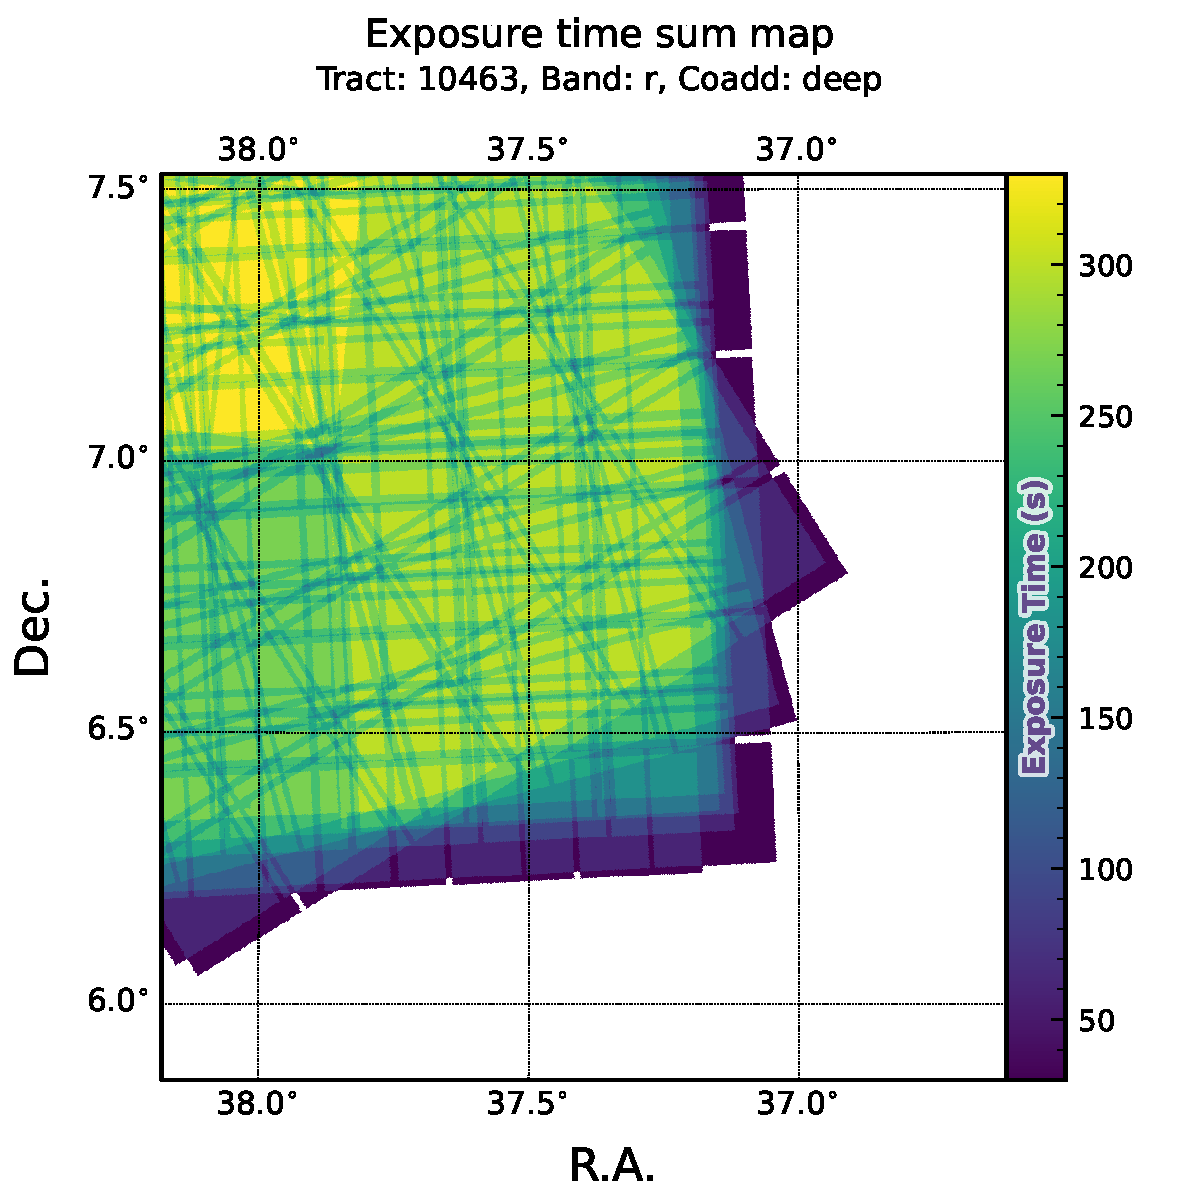
\includegraphics[width=\linewidth, height=5.8cm]{deepCoadd_exposure_time_map_sum_tract10463_rband.pdf}
  \caption{Total exposure time sum map for   \texttt{deep\_coadd} \gls{tract} 10463, band: r in field Rubin\_SV\_38\_7}
  \end{subfigure}\hfill
  \begin{subfigure}[t]{0.31\textwidth}
  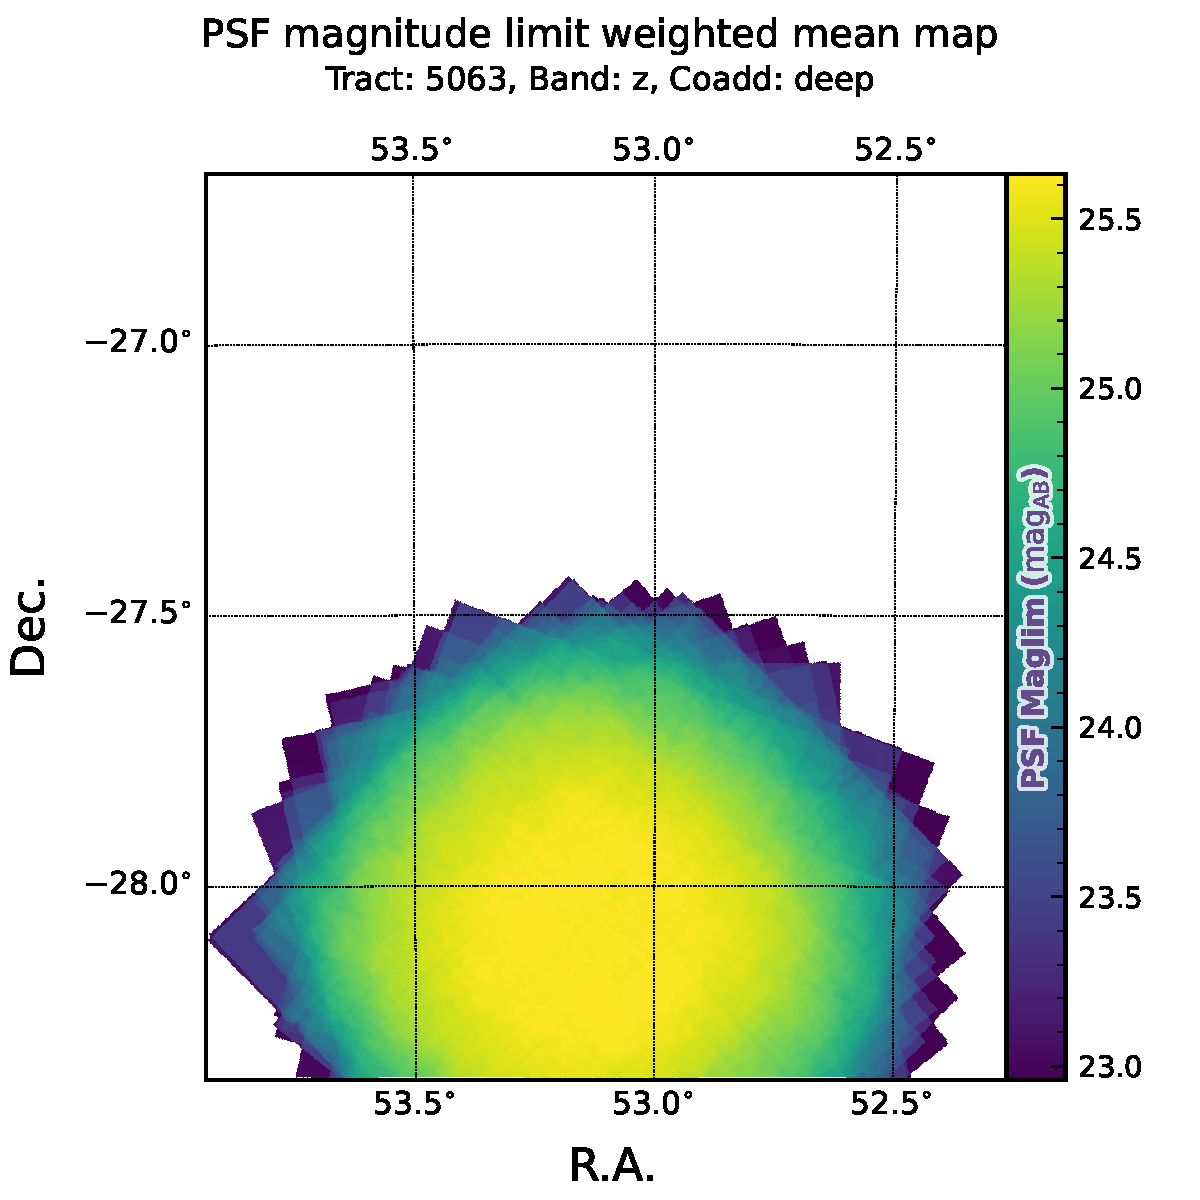
\includegraphics[width=\linewidth, height=5.8cm]{deepCoadd_psf_maglim_map_weighted_mean_tract5063_zband.pdf}
  \caption{5$\sigma$ \gls{PSF} magnitude limit weighted mean map for \texttt{deep\_coadd} \gls{tract} 5063, band z in field ECDFS}
  \end{subfigure}\hfill
    \begin{subfigure}[t]{0.31\textwidth}
  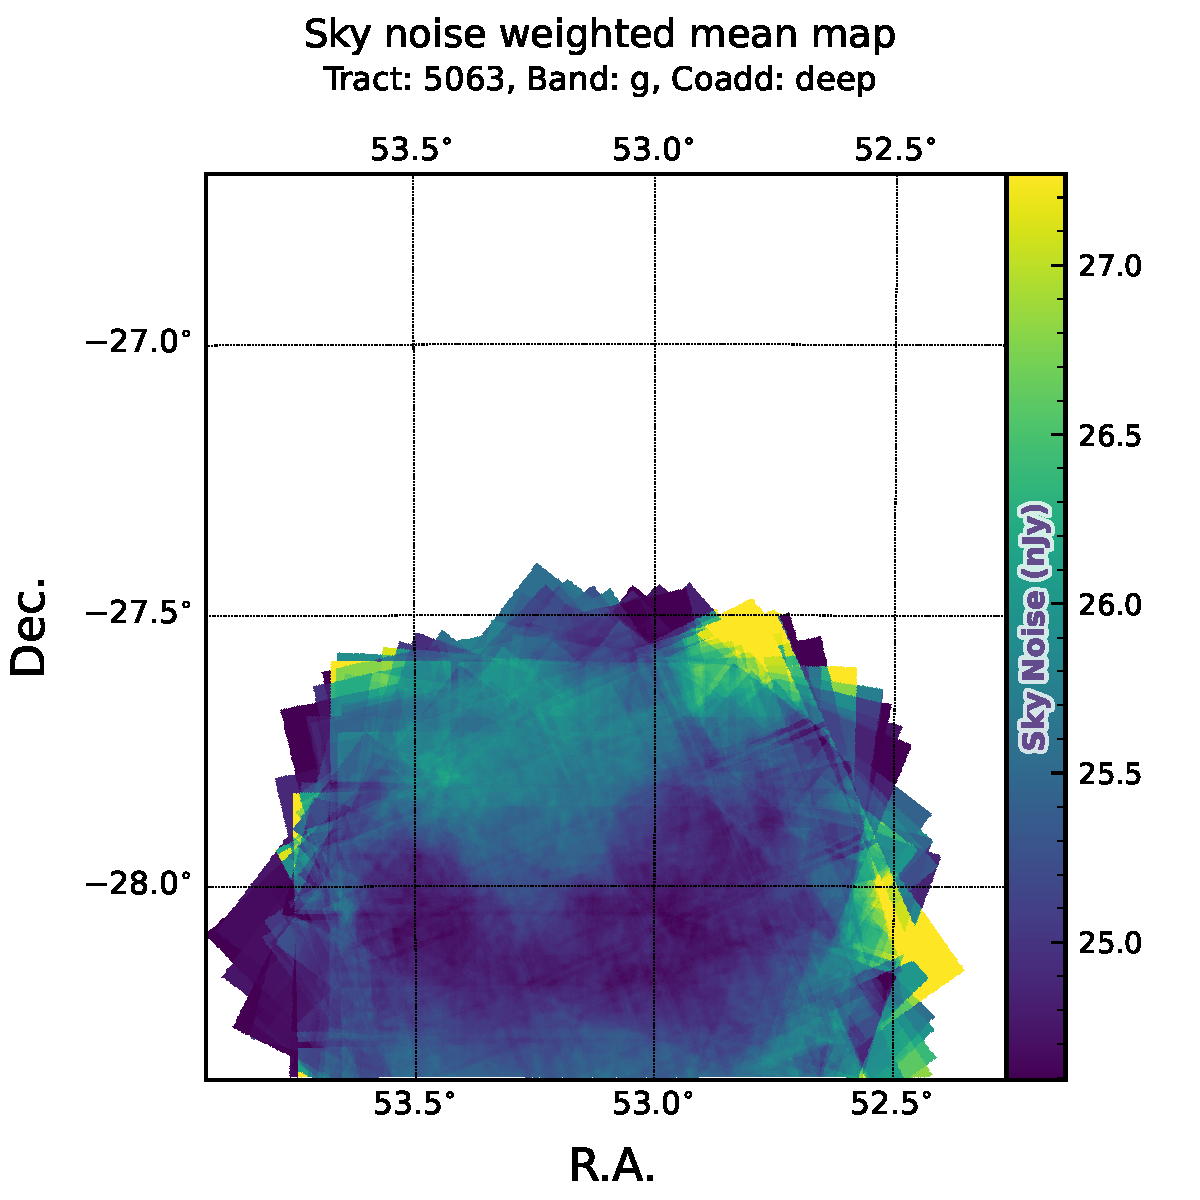
\includegraphics[width=\linewidth, height=5.8cm]{deepCoadd_sky_noise_map_weighted_mean_tract5063_gband.pdf}
  \caption{Sky noise weighted mean map for \texttt{deep\_coadd} \gls{tract} 5063, band z in ield ECDFS}
  \end{subfigure}\hfill
\caption{Examples of survey property maps from Rubin \gls{DP1} across different bands, clipped to the boundary of a single \gls{tract} for visual clarity.}
  \label{fig:survey_property_maps}
\end{figure*}

% HiPS maps
% Leanne: updated to state that single-band will only come post-DP1 release
\subsubsection{HiPS Maps}
% Rephrase to avoid 'DP1' twice
\gls{HiPS} Maps \citep{2015A&A...578A.114F}, offer an interactive way to explore seamless, multi-band tiles of the sky regions covered by \gls{DP1}, allowing for smooth panning and zooming.
\gls{DP1} provides multi-band \gls{HiPS} images created by combining data from individual bands of \texttt{deep\_coadd} and \texttt{template\_coadd} images.
These images are false-color representations generated using various filter combinations for the red, green, and blue channels.
The available filter combinations include \textit{gri}, \textit{izy}, \textit{riz}, and \textit{ugr} for both \texttt{deep\_coadd} and \texttt{template\_coadd}.
Additionally, for \texttt{deep\_coadd} only, we provide color blends such as \textit{uug} and \textit{grz}.
Post-\gls{DP1}, we plan to also provide single-band HiPS images for all $ugrizy$ bands in both \gls{PNG} and \gls{FITS} formats.

\gls{HiPS} maps are only accessible through the \gls{HiPS} viewer in the \gls{RSP} Portal (\secref{ssec:rsp_portal}) and cannot be accessed via the Data \gls{Butler} (\secref{sssec:data_butler}).
All multi-band \gls{HiPS} images are provided in \gls{PNG} format.

% Visit summary table.
%visitSummaryTable == visit_table = Visit (TAP)
% visitDetectorSummaryTable ==visit_detector_table == CCDVisit?
\subsection{Metadata
\label{ssec:metadata}}
%Here we describe metadata tables produced by the Observatory directly and not the science pipelines

\gls{DP1} also includes \gls{metadata} about the observations, which is stored in the \texttt{Visit} table. The data it contains is produced by the observatory directly, rather than the science pipelines.
It contains technical data for each visit, such as telescope pointing, \gls{camera} rotation, \gls{airmass}, exposure start and end time, and total exposure time.

%Since the \texttt{Visit} table is generated by the processing pipelines it only includes entries for visits that successfully passed processing.
%DP1 contains \nvisitsummarytables \texttt{visit\_table} summarizing data for a total of  \nvisitsummaries visits.

% The \texttt{visit\_table} sits outside the \texttt{tract} and \texttt{visit}-level convention.

%Visit table in qserv as well - this should be the primary interface to query images. And...In future releases, the visit summary table will also be available over TAP, allowing users to execute queries selecting on on a wider range of attributes, such as seeing.

% As above - I think this is obvious and can delete
% The \texttt{visit\_detector\_table} sits outside the \texttt{tract} and \texttt{visit}-level convention.
%\james{Why is the number of rows in the visit-detector summary table (\nvisitdetectorsummaries) not the same as either the number of raw images ({\nraws}) or the number of visit images (\nvisitimages)?!}

\subsection{Ancillary Data Products
\label{subsec:ancilliary}}
DP1 also includes several ancillary data products. While we do not expect most users to need these, we describe them here for completeness. All the Data Products described in this section can only be accessed via the Data Butler (\secref{sssec:data_butler}).

\subsubsection{Task configuration, log, and metadata}
\gls{DP1} includes \gls{provenance}-related data products such as task logs, \gls{configuration} files, and task metadata.
Configuration files record the parameters used in each processing task, while logs and \gls{metadata} contain information output during processing. These products help users understand the processing setup and investigate potential processing failures.
%They can be visit-level, tract-level, or neither, depending on the task.
% The method for uniquely referencing a data product also depends on the task.

\subsubsection{Pipeline-generated plots and metrics}
\gls{DP1} includes various plots and metrics generated during data processing, such as  plots comparing measured fluxes and source positions relative to references, and metrics indicating the numbers of flagged pixels in a given \texttt{visit\_image}. These data products are predominantly used by the data management team to assess the quality of the processed data. We include them with \gls{DP1} for transparency.

% Leanne -- reviewed by Chris ZW
\subsubsection{Calibration Data Products}
\label{ssec:calibration_data}
Calibration data products include a variety of images and models that are used to characterize and correct the performance of the \gls{camera} and other system components.
These include bias, dark, and flat-field images, \gls{PTC} gains, brighter-fatter kernels, charge transfer inefficiency (\gls{CTI}) models, linearizers, and illumination corrections.
For flat-field corrections, \gls{DP1} processing used combined flats, which are averaged from multiple individual flat-field exposures to provide a stable \gls{calibration}. These \gls{calibration} products are essential inputs to \gls{ISR} (\secref{ssec:isr}). While these products are included in \gls{DP1} for transparency and completeness, users should not need to rerun ISR for their science and are advised to start with the processed \texttt{visit\_image}.

\subsubsection{Standard Bandpasses}
\label{ssec:bandpasses_dataproducts}
The \texttt{standard\_passband} data products contain the system throughputs described in \secref{sssec:comcam_filters}.

% \tabref{tab:calibration_data_products} lists the calibration data products in DP1, their associated Butler dataset types, and describes the issues each addresses and the order in which they are applied.. which flat? combined? certified?
% % Table X lists the calibration data priducts abd  the issue they address sorted in teh  in the order applied to ISR. 2 scolumns, Product and Issue.
\begin{deluxetable}{lcc}
\caption{DP1 Calibration Data Products  with the corresponding butler dataset type. \label{tab:calibration_data_products}}
\tablehead{
\colhead{Data Product} & \colhead{Type} & \colhead{Description}
}
\startdata
LSSTComCam & Instrument &\texttt{camera}  \\ 
Photon Transfer Curve & & \texttt{ptc}  \\ 
Brighter Fatter Kernel & image & \texttt{raw}   \\
Dark & image  & \texttt{dark}    \\ 
Flat & image  & \texttt{flat}   \\ 
Bias & image  & \texttt{bias}   \\ 
Defects & map  & \texttt{defects}   \\ 
Linearizer &<?> & \texttt{linearizer}   \\ 
\enddata
\end{deluxetable}

% Check if we are providing any files and if not, remove
%\subsection{Files}
%\label{subsec:files}
%\james{Are we providing any files?}

%Parquet Files -- check if we are providing them. remove if not

%FITS files -- are we providing these? Probably not
